
\documentclass{standalone}
\usepackage{tikz}
\usepackage{standalone}
\usetikzlibrary{calc}
\begin{document}
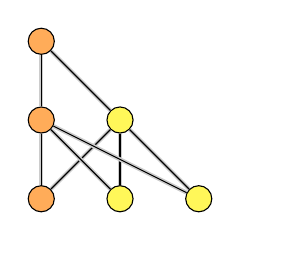
\begin{tikzpicture}
\node[circle, draw=black, fill=orange!65, label={[xshift=.5cm, yshift=-.55cm]\textcolor{white}{\tiny{0.5}}}] (0) at (0, 0) {};
\node[circle, draw=black, fill=yellow!65, label={[xshift=.5cm, yshift=-.55cm]\textcolor{white}{\tiny{0.6}}}] (1) at (1, 0) {};
\node[circle, draw=black, fill=yellow!65, label={[xshift=.5cm, yshift=-.55cm]\textcolor{white}{\tiny{0.4}}}] (2) at (2, 0) {};
\node[circle, draw=black, fill=orange!65, label={[xshift=.5cm, yshift=-.55cm]\textcolor{white}{\tiny{0.6}}}] (3) at (0, 1) {};
\node[circle, draw=black, fill=yellow!65, label={[xshift=.5cm, yshift=-.55cm]\textcolor{white}{\tiny{0.2}}}] (4) at (1, 1) {};
\node[circle, draw=black, fill=orange!65, label={[xshift=.5cm, yshift=-.55cm]\textcolor{white}{\tiny{0.2}}}] (5) at (0, 2) {};

\draw[line width=1.5pt,-,black!20] (0) -- (3);
\draw[draw,-] (0) -- (3);
\draw[line width=1.5pt,-,black!20] (0) -- (4);
\draw[draw,-] (0) -- (4);
\draw[line width=1.5pt,-,black!20] (1) -- (3);
\draw[draw,-] (1) -- (3);
\draw[line width=1.5pt,-,black!20] (1) -- (4);
\draw[draw,-] (1) -- (4);
\draw[line width=1.5pt,-,black!20] (2) -- (3);
\draw[draw,-] (2) -- (3);
\draw[line width=1.5pt,-,black!20] (2) -- (4);
\draw[draw,-] (2) -- (4);
\draw[line width=1.5pt,-,black!20] (3) -- (5);
\draw[draw,-] (3) -- (5);
\draw[line width=1.5pt,-,black!20] (4) -- (5);
\draw[draw,-] (4) -- (5);
\end{tikzpicture}
\end{document}